
%----------------------------------------------------------------------
\begin{frame}
\frametitle{\code{Array} class}

\begin{itemize}
\item Conceptually a Fortran-like array
\item Data distributed via MPI-[12], OMP, [UPC]
\item Data layout may be blocked / padded for cache
\item Interface between high-level C++ and low-level Fortran/C
\end{itemize}
\end{frame}

%----------------------------------------------------------------------
\begin{frame}
\frametitle{\code{Array} class}

\begin{minipage}{1.8in}
\begin{itemize}
\item[]\enhance{1-}
\includegraphics[width=0.4in]{array-serial.png} \ \ \code{ArraySerial}
\item[]\enhance{2-}
\includegraphics[width=0.4in]{array-block.png} \ \ \code{ArrayBlock}
\item[]\enhance{3-}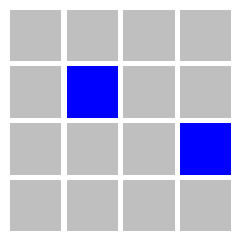
\includegraphics[width=0.4in]{array-mpi.png} \ \ \code{ArrayMpi}
\end{itemize}
\end{minipage} \ 
\begin{minipage}{2in}
\begin{itemize}
\item[]\enhance{4-}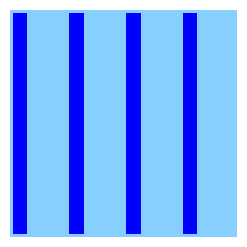
\includegraphics[width=0.4in]{array-omp.png} \ \ \code{ArrayOmp}
\item[]\enhance{5-}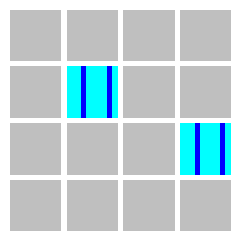
\includegraphics[width=0.4in]{array-mpi-omp.png} \ \ \code{ArrayMpiOmp}
\item[]\enhance{6-}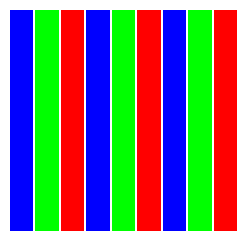
\includegraphics[width=0.4in]{array-interleave.png} \ \ \code{ArrayInterleave}
\end{itemize}
\end{minipage}

\end{frame}
%----------------------------------------------------------------------
